\documentclass[12pt, letterpaper]{article}

\title{CS302: Trees}
\author{Amiel L. Iliesi}
\date{2026-04-08}

% packages
\usepackage[hidelinks]{hyperref}
\usepackage[x11names]{xcolor}
\usepackage{graphicx}

% new commands
\newcommand{\question}[2][4em]{\textbf{#2}\vspace{#1}\par}
\newcommand{\answer}[1]{\color{Green4}\textbf{#1}\normalcolor}

% new environments
\newenvironment{answerblock}{\color{Green4}}{\normalcolor\vspace{1em}}

% global settings
\setlength{\parindent}{0pt}
\setlength{\parskip}{0.5em}
\graphicspath{{./figures/}}

\begin{document}

\maketitle

\tableofcontents

\pagebreak
\section{Trees in General}

\question{In your words, describe a tree. Include all properties that
\emph{all} trees \emph{must} have.}

\question[12em]{Describe the following terms: depth, height, balanced, full tree, complete tree.}

\question{What makes iterating on trees so difficult? What is the solution?}

\question{Can you give an example of a most basic type of tree; an unordered,
n-child tree.}

\pagebreak
\section{Ordered Trees}

\subsection{Properties}

\question{What makes ordered trees different? State their required
properties/invariants.}

\question[0em]{Is the following binary tree ordered? Explain your answer.}

\begin{center}
    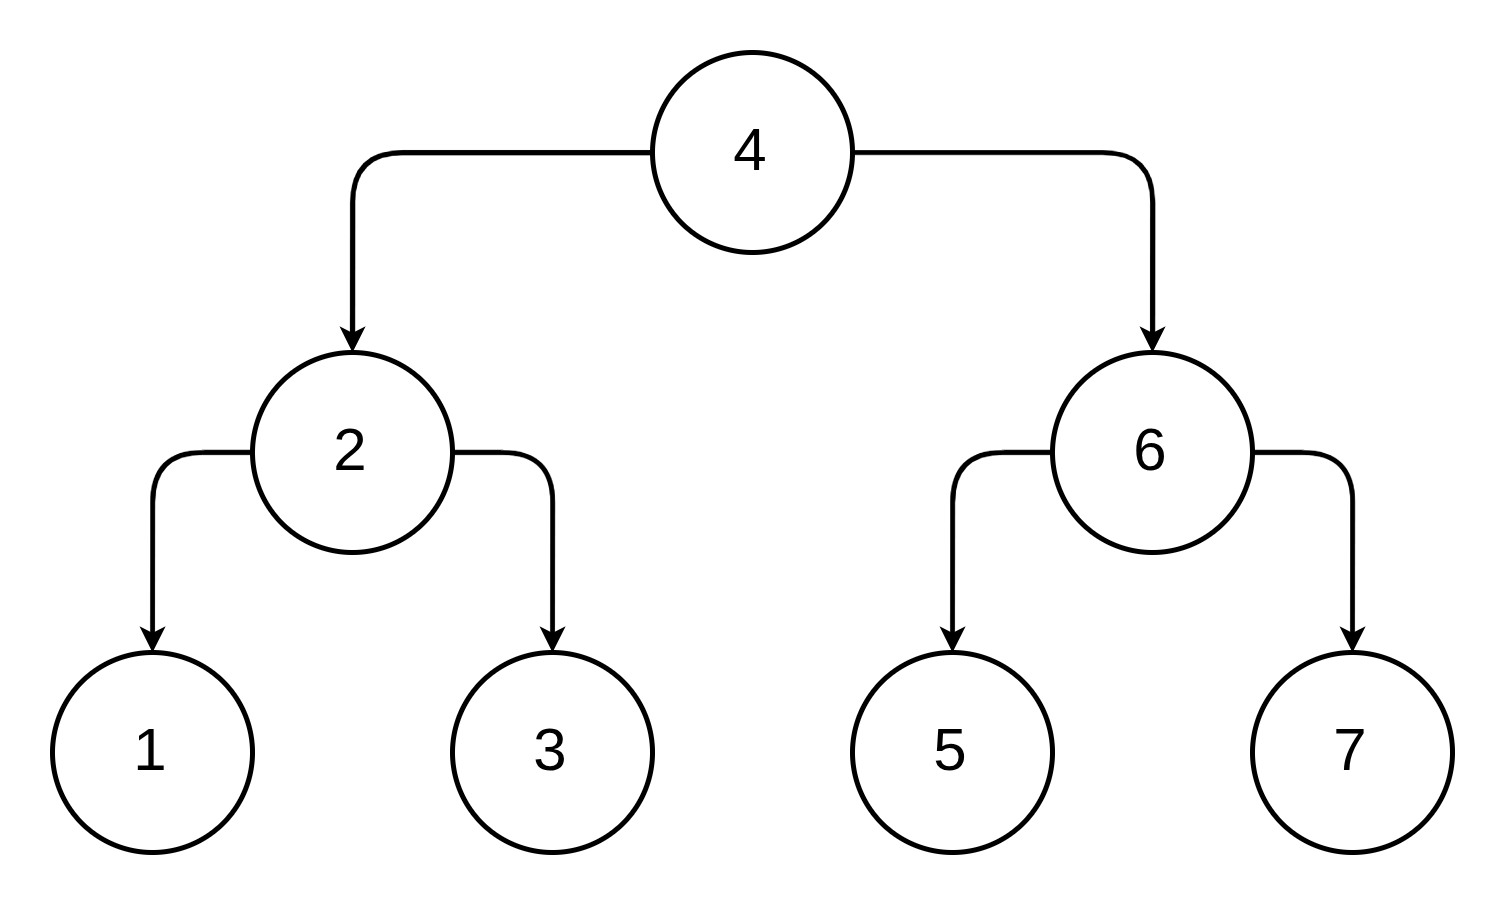
\includegraphics[width=0.5\textwidth]{ordered_tree(1).png}
\end{center}

\vspace{8em}

\begin{minipage}{\textwidth}
\question[0em]{Is the following binary tree ordered? Explain your answer.}

\begin{center}
    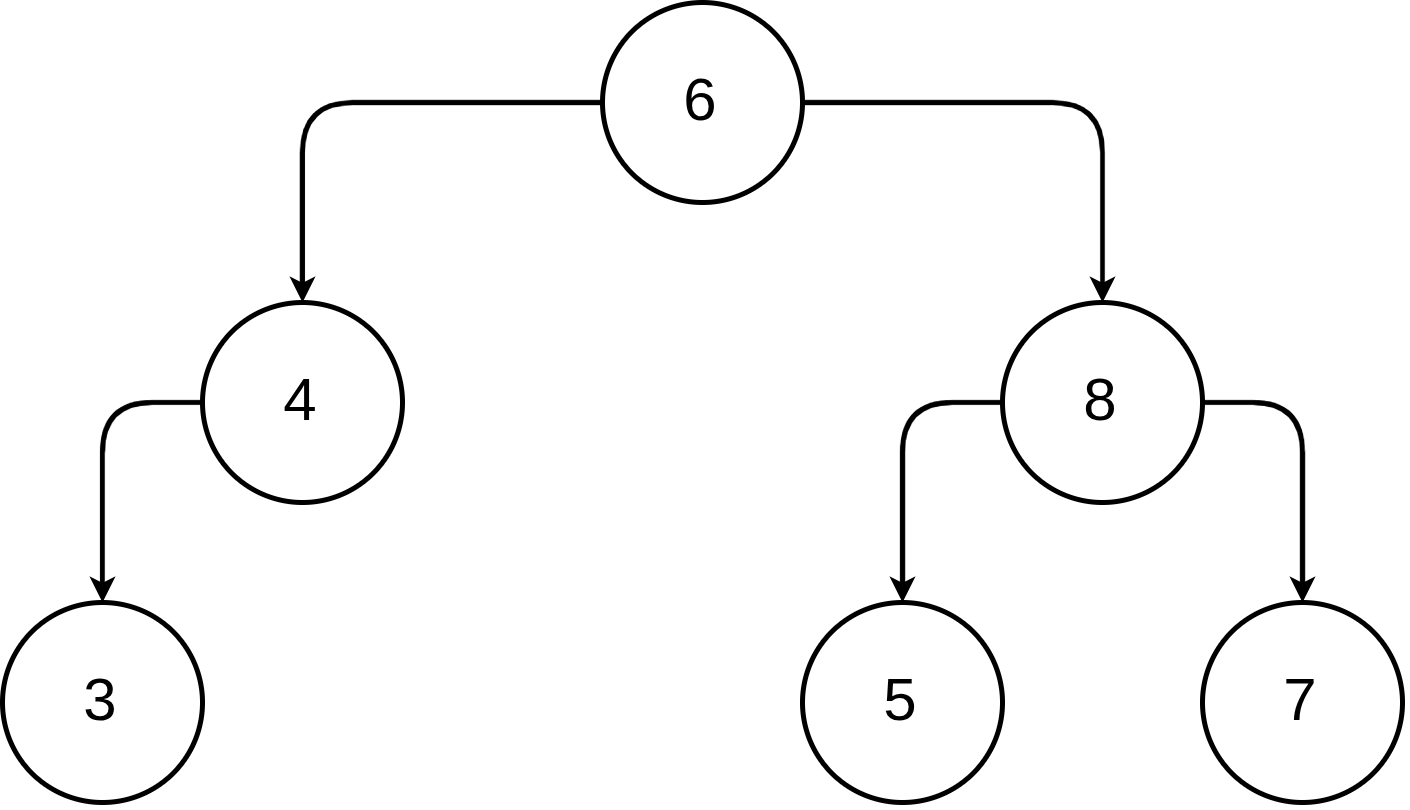
\includegraphics[width=0.5\textwidth]{ordered_tree(2).png}
\end{center}

\vspace{8em}
\end{minipage}

\subsection{Implementation}

\question{Describe the process of adding a new integer into an unbalanced,
binary search tree.}

\question{Describe the process of removing an integer from an unbalanced,
binary search tree.}

\pagebreak
\section{Balanced vs Unbalanced}

\question{What is a self-balancing tree? Describe a situation where you would
prefer a self-balancing tree, and a situation where you might not prefer one.}

\subsection{Types}

\textbf{Describe each of the types below, and what makes them unique. List any
invariants they may have as well.}

\question{Red-Black Tree:}

\question{2-3-4 Tree:}

\question{Heap:}

\question{B-Tree:}

\end{document}